\section{The TMS-1000}
\begin{frame}
	  \frametitle{Der erste Mikrocontroller - System-on-a-Chip}
	  \begin{center}

		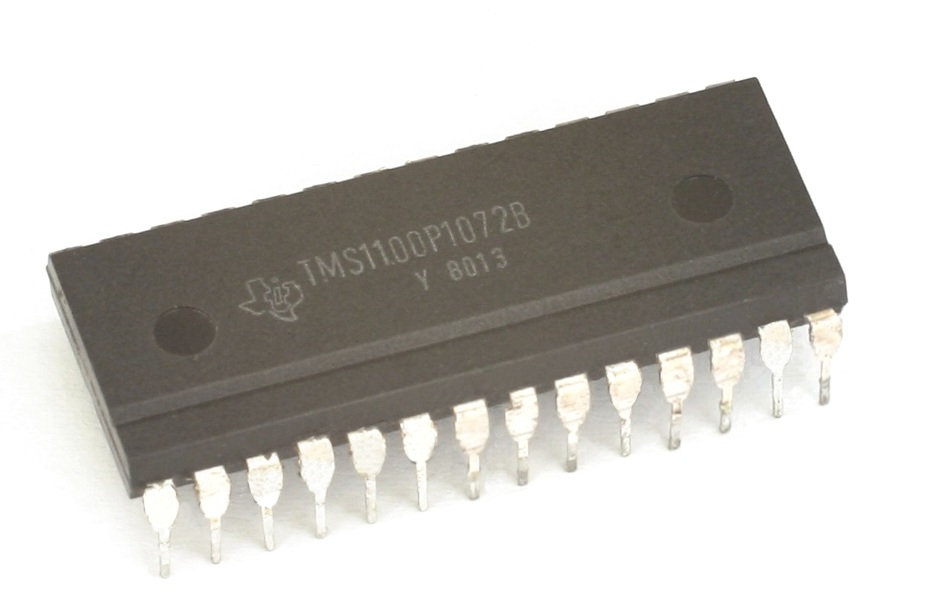
\includegraphics[scale=0.25]{images/KL_TI_TMS1100.jpg}


	  \end{center}
\end{frame}


\begin{frame}
	\frametitle{Inhalt}
		\begin{enumerate}
			\item Geschichte \pause
			\item Mikrokontroller allgemein \pause
			\item TMS1000 \pause \begin{itemize}
										\item Allgemeine Daten \pause
										\item Aufbau \& Funktionsweise \pause
										\item Befehlssatz \pause
										\end{itemize}
			\item Verwendung des TMS1000
		\end{enumerate}
\end{frame}

\subsection{Geschichte}
\begin{frame}
	\frametitle{Entstehung}
		\begin{itemize}
			\item Entwickelt von Gary Boone \& Michael Cochran 1971 \pause
			\item Zuerst von Texas Instrument verwendet \pause
			\item Erst 1974 auf dem freien Markt erh{\"a}ltlich \pause
			\item Bis heute ca. 100 Millionen verkaufte Exemplare 
		\end{itemize}
\end{frame}

\subsection{Mikrokontroller allgemein}
\begin{frame}
	\frametitle{Miktrokontroller allgemein}
		\begin{center}
		{\huge Aufbau:}
		\end{center}
		\begin{itemize}
		\item CPU - Prozessor \pause
		\item RAM - Arbeitsspeicher \pause
		\item ROM - Festspeicher \pause 
		\item Takt \pause
		\item Peripherie - I/O-Ports
		\end{itemize}
\end{frame}

\subsection{Der TMS-1000}
\begin{frame}
	\frametitle{Allgemeine Daten - TMS1000}
		\framesubtitle{Abbildung der Pins}
\begin{figure}
	\centering
		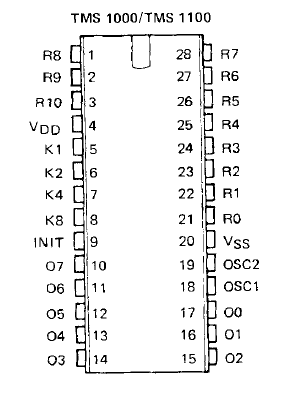
\includegraphics[scale=0.5]{images/pins.PNG}
\end{figure}

\end{frame}

\begin{frame}
	\frametitle{Allgemeine Daten - TMS1000}
	\begin{itemize}
		\item ROM: 1024x8 Bits \pause
		\item RAM: 64x4 Bits \pause
		\item 43 Basis Instruktionen \pause
		\item Max. Spannung 20V \pause
		\item H{\"o}chste erreichbare Frequenz: 0,4MHz
	\end{itemize}
\end{frame}


\begin{frame}
	\frametitle{Aufbau \& Funktionsweise}
		\framesubtitle{Schaltbild des TMS-1000}
\begin{figure}
	\centering
		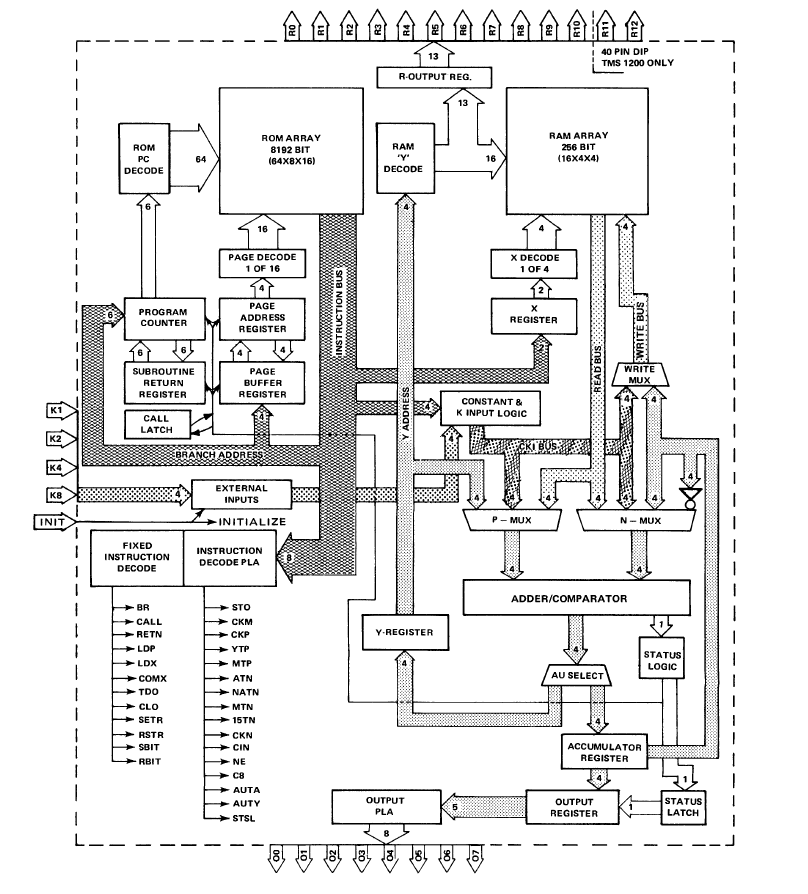
\includegraphics[scale=0.28]{images/schaltbild.PNG}
\end{figure}
\end{frame}

\begin{frame}
\frametitle{Aufbau \& Funktionsweise}
	  \framesubtitle{ROM}
		 \begin{columns}
      \begin{column}{5cm}
    		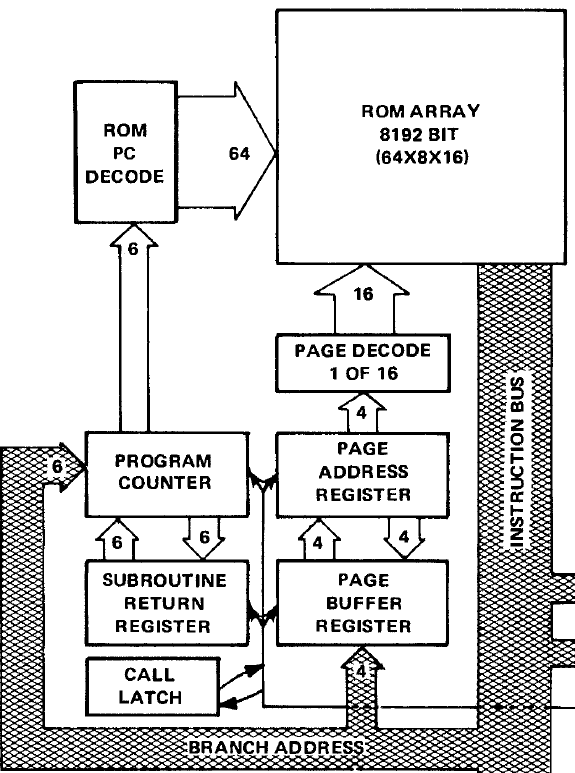
\includegraphics[scale=0.3]{images/ROM.PNG}
      \end{column}
      \begin{column}{5cm}
       \begin{itemize}
        \item 16 Seiten je 64 W{\"o}rter \pause
        \item 3 Register die den ROM adressieren \pause
        \item Page Adress (PA) \pause
        \item Page Buffer (PB) \pause
        \item Program Counter (PC)
       \end{itemize}
      \end{column}
     \end{columns}
\end{frame}

\begin{frame}
\frametitle{Aufbau \& Funktionsweise}
 \framesubtitle{Branching \& Subroutines}
 		 \begin{columns}
      \begin{column}{5cm}
    		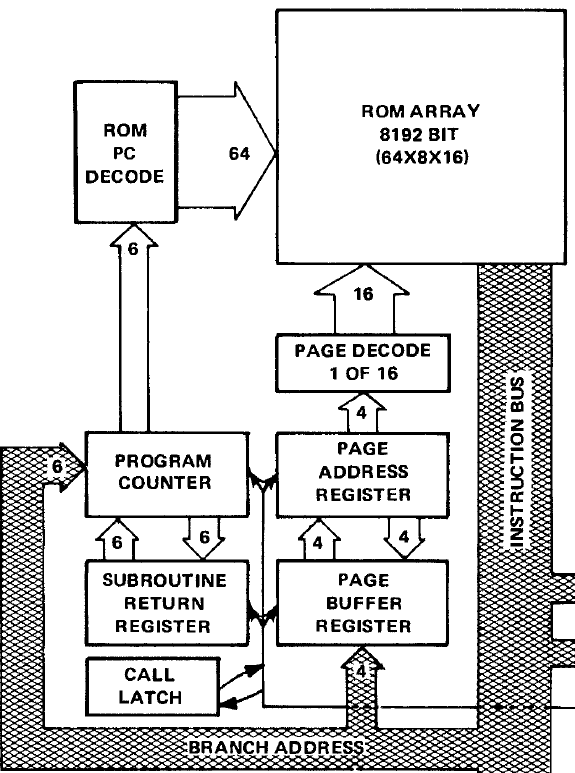
\includegraphics[scale=0.3]{images/ROM.PNG}
      \end{column}
      \begin{column}{5cm}
        	\begin{itemize}
 						\item Conditional \pause
 						\item ALU setzt Status-Logic Bit \pause
 						\item Standardm{\"a}{\ss}ig auf 1
 					\end{itemize}
      \end{column}
     \end{columns}
\end{frame}


\begin{frame}
\frametitle{Aufbau \& Funktionsweise}
	\framesubtitle{RAM}
		\begin{columns}
			\begin{column}{5cm}
				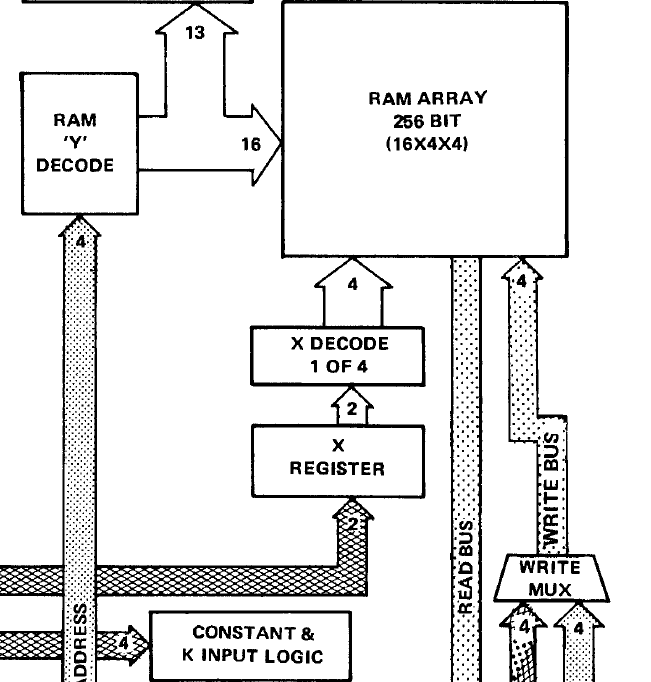
\includegraphics[scale=0.3]{images/RAM.PNG}
			\end{column}
			\begin{column}{5cm}
				\begin{itemize}
					\item 4 Dateien mit je 16 W{\"o}rtern \pause
					\item Wird durch X und Y Register adressiert \pause
					\item X adressiert "`Seite"', Y das Wort \pause
					\item Input durch Write-Multiplexer \pause
					\item Output durch Read-Bus
				\end{itemize}
			\end{column}
		\end{columns}
\end{frame}

\begin{frame}
\frametitle{Aufbau \& Funktionsweise}
	\framesubtitle{Constant and K Input (CKI) Logic}
		\begin{columns}
			\begin{column}{5cm}
				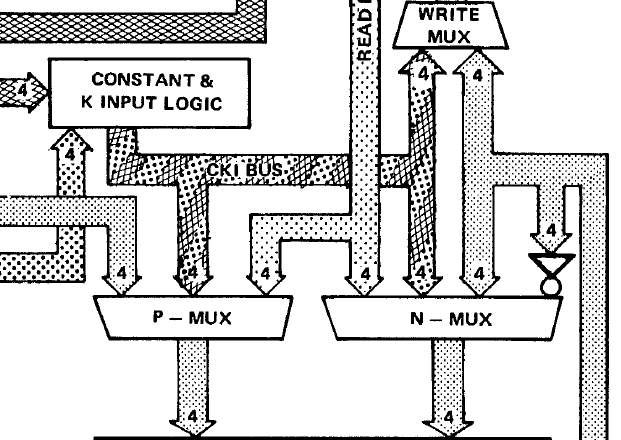
\includegraphics[scale=0.3]{images/CKI.PNG}
			\end{column}
		\begin{column}{5cm}
			\begin{itemize}
				\item Verwendet entweder K-Inputs oder Konstanten aus dem ROM \pause
				\item Kann entwededer in P-MUX, N-MUX oder RAM schreiben
			\end{itemize}
		\end{column}
	\end{columns}
\end{frame}


\begin{frame}
\frametitle{Aufbau \& Funktionsweise}
	\framesubtitle{Y-Register}
		\begin{itemize}
			\item Adressiert RAM \pause
			\item Setzt R-Output Latches
		\end{itemize}
\end{frame}


\begin{frame}
	\frametitle{R-Output}
		\begin{itemize}
			\item Externe Ger{\"a}te \pause
			\item	Display Scans \pause
			\item Input Encoding \pause
			\item Status Logic Outputs
		\end{itemize}
\end{frame}


\begin{frame}
\frametitle{Aufbau \& Funktionsweise}
	\framesubtitle{Akkumulator \& ALU}
		\begin{columns}
			\begin{column}{5cm}
				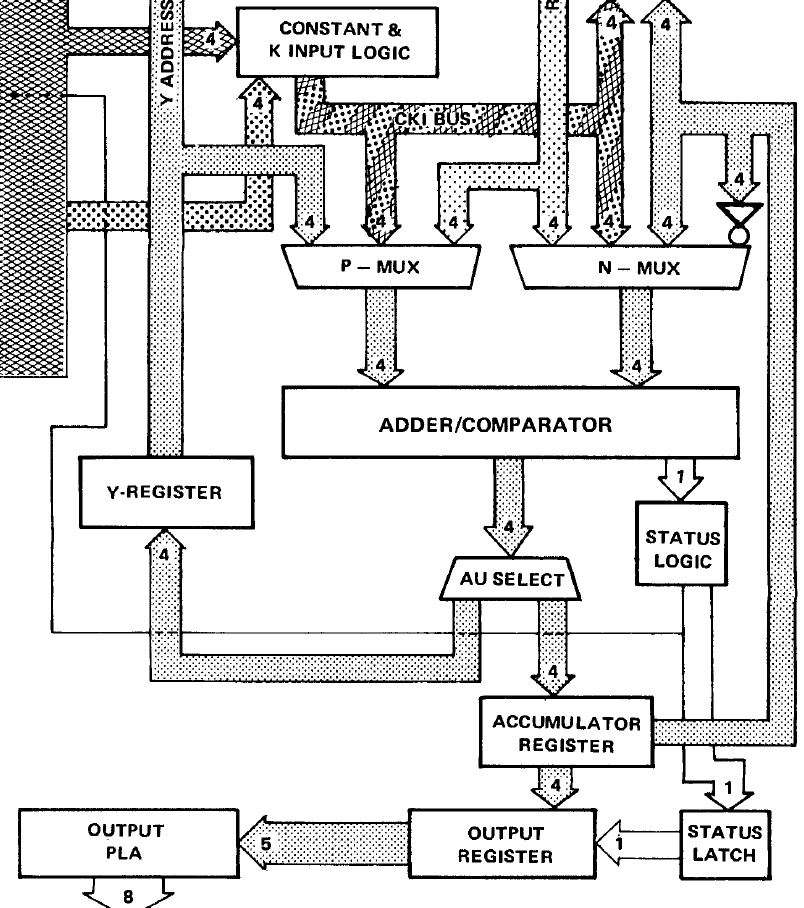
\includegraphics[scale=0.25]{images/ALU.PNG}
			\end{column}
			\begin{column}{5cm}
				\begin{itemize}
					\item 4-Bit Adder/Comperator \pause
					\item Kann addieren, subtrahieren und logische Vergleiche \pause
					\item Addition/Substraktion entweder im Y-Register oder Akkumulator gespeichert \pause
					\item Ergebnis Vergleiche im Status-Logic-Bit
				\end{itemize}
			\end{column}
		\end{columns}
\end{frame}
	

\begin{frame}
\frametitle{Aufbau \& Funktionsweise}
	\framesubtitle{O-Output}
		\begin{columns}
			\begin{column}{5cm}
				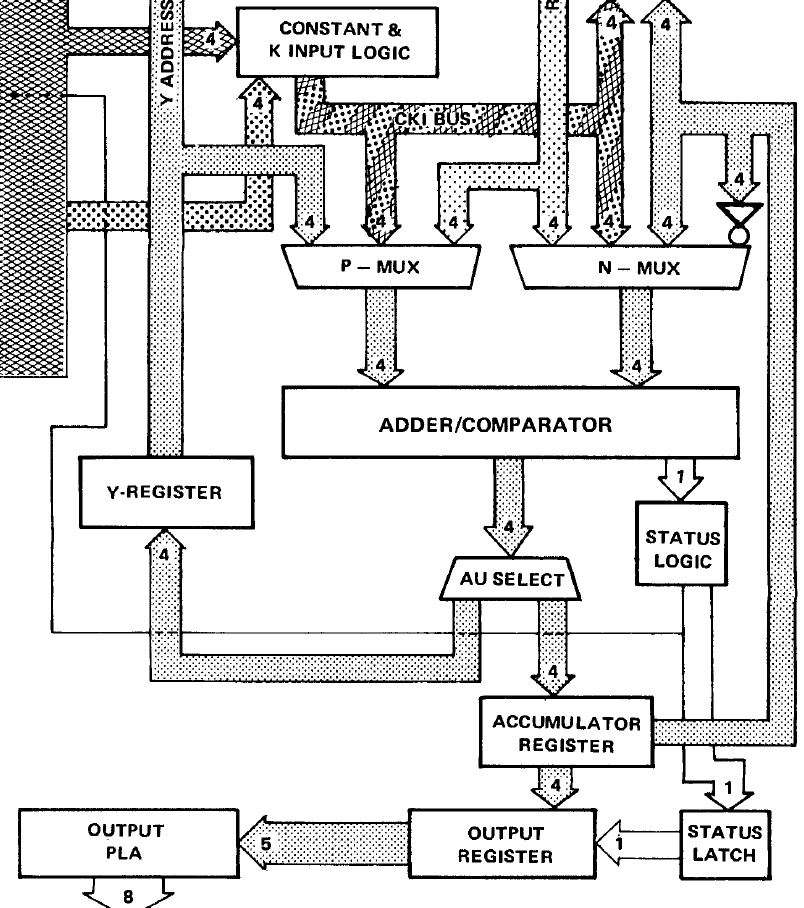
\includegraphics[scale=0.25]{images/ALU.PNG}
			\end{column}
			\begin{column}{5cm}
				\begin{itemize}
					\item Gibt Akkumulator und Status-Bit aus \pause
					\item PLA kodiert 5 Input-Bits in 8 Ausg{\"a}nge
				\end{itemize}
			\end{column}
		\end{columns}
\end{frame}

\begin{frame}
\frametitle{Aufbau \& Funktionsweise}
	\framesubtitle{Instruction-Decoder}
		\begin{columns}
			\begin{column}{5cm}
				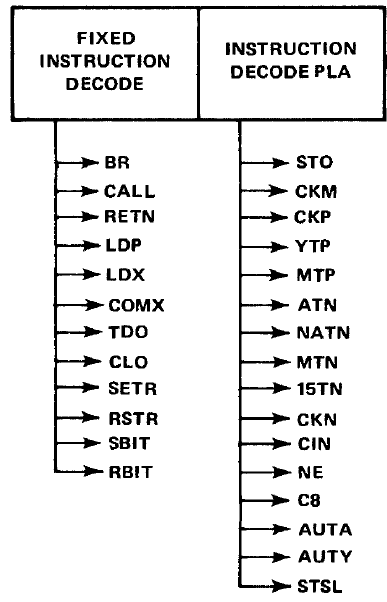
\includegraphics[scale=0.3]{images/IDEC.PNG}
			\end{column}
			\begin{column}{5cm}
				\begin{itemize}
					\item 12 feste Instruktionen \pause
					\item 31 programmierbare Instruktionen \pause
					\item Sind standardm{\"a}{\ss}ig definiert, k{\"o}nnen aber abge{\"a}ndert werden \pause
					\item PLA kombiniert die 16 Mikroinstruktionen zu einem Ausdruck
				\end{itemize}
			\end{column}
		\end{columns}
\end{frame}


\begin{frame}
\frametitle{Aufbau \& Funktionsweise}
	\framesubtitle{INIT-Pin}
		\begin{itemize}
			\item Initialisiert die Hardware \pause
			\item Resettet PA, PC und die R- \& O-Output Register
		\end{itemize}
\end{frame}


\begin{frame}
\frametitle{Aufbau \& Funktionsweise}
	\framesubtitle{Befehlssatz}
		\begin{figure}
			\centering
				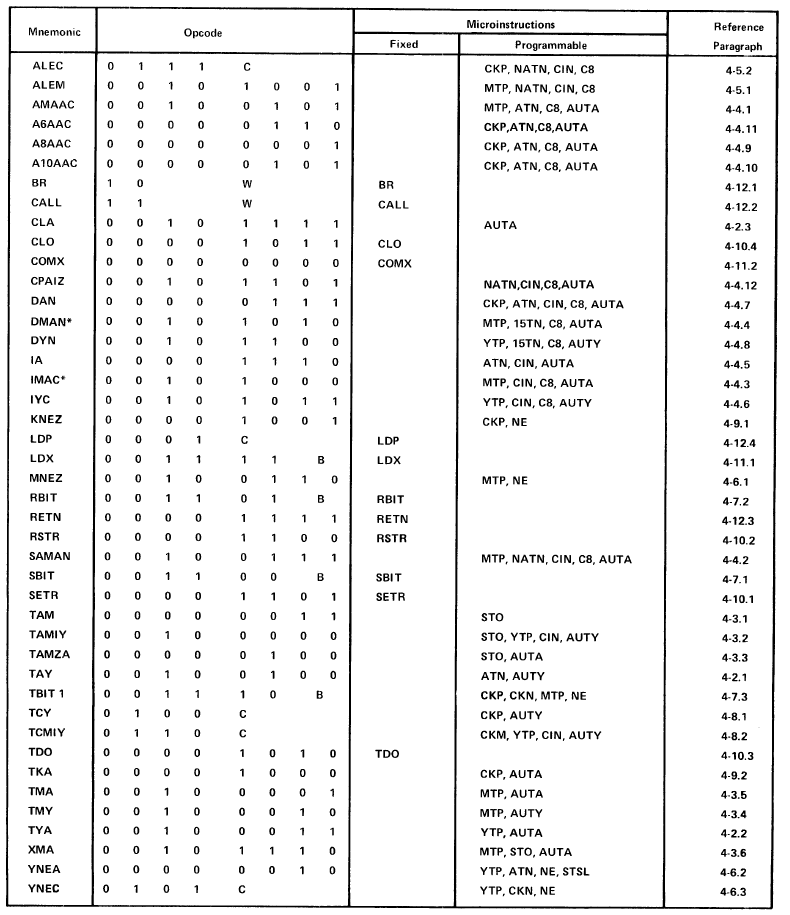
\includegraphics[scale=0.25]{images/INSTRUCT.PNG}
		\end{figure}
\end{frame}


\begin{frame}
\frametitle{Aufbau \& Funktionsweise}
	\framesubtitle{Instruktions-Formate}
		\begin{center}
			Format 1: \\
			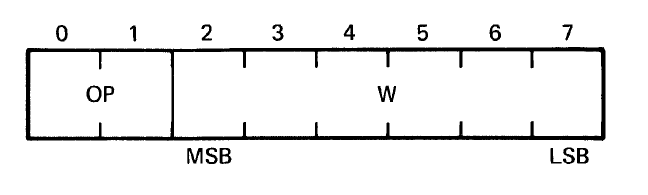
\includegraphics[scale=0.25]{images/I1.PNG} \\ \pause
			Format 2: \\
			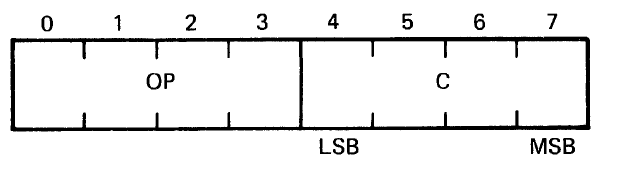
\includegraphics[scale=0.25]{images/I2.PNG} \\ \pause
			Format 3: \\
			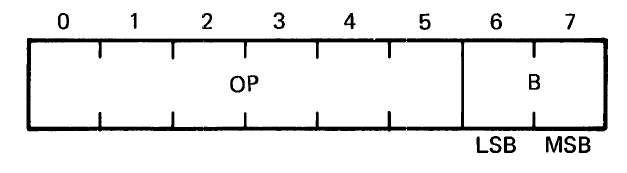
\includegraphics[scale=0.25]{images/I3.PNG} \\ \pause
			Format 4: \\
			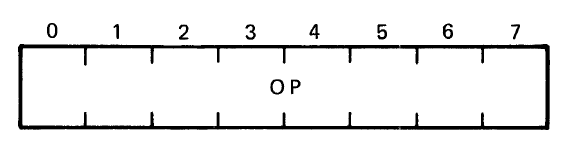
\includegraphics[scale=0.25]{images/I4.PNG} \\ 
		\end{center}
\end{frame}


\begin{frame}
\frametitle{Aufbau \& Funktionsweise}
	\framesubtitle{Beispiel: AMAAC}
		\begin{itemize}
			\item Add Memory to Accumulator, Result to Accumulator \pause
			\item Format: 4 \pause
			\item Mikroinstruktionen: MTP, ATN, C8, AUTA \pause
			\item M(X,Y) + A in A \pause
			\item Carry = 1 falls Summe gr{\"o}{\ss}er 15
		\end{itemize}
\end{frame}

\begin{frame}
\frametitle{Aufbau \& Funktionsweise}
	\framesubtitle{Beispiel: SAMAN}
		\begin{itemize}
			\item Substract Accumulator from Memory, Result to Accumulator \pause
			\item Format: 4 \pause
			\item Mikroinstruktionen: MTP, NATN, CIN, C8, AUTA \pause
			\item M(X,Y) - A in A \pause
			\item Carry = 0 falls A gr{\"o}{\ss}er M(X,Y)
		\end{itemize}
\end{frame}

\begin{frame}
\frametitle{Aufbau \& Funktionsweise}
	\framesubtitle{Beispielprogramm}
		\begin{figure}
			\centering
				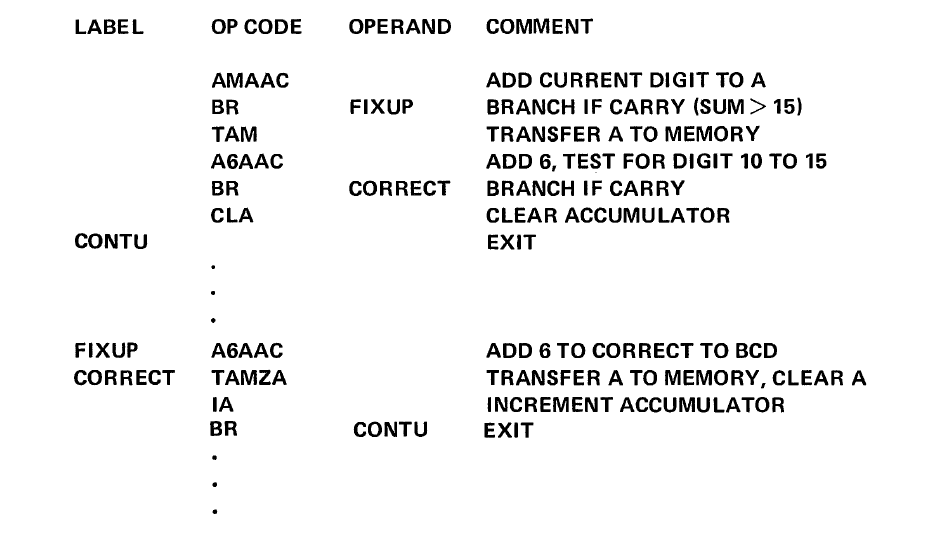
\includegraphics[scale=0.3]{images/BSPProg.PNG}
		\end{figure}
\end{frame}

\subsection{Verwendung Mikrocontroller}
\begin{frame}
	\frametitle{Verwendung}
		\begin{itemize}
			\item In eingebetteten Systemen \pause
			\item In Leistung und Austattung meist auf eine Anwendung angepasst \pause
			\item Beispiele: Unterhaltungselektronik, Waschmaschinenen, Steuerger{\"a}te, uvm. \pause
			\item TMS1000: Taschenrecher, wie z.B SR-16
		\end{itemize}
\end{frame}

\begin{frame}
\frametitle{Verwendung}
	\framesubtitle{Der SR-16}
	\begin{columns}
		\begin{column}{5cm}
			\centering
				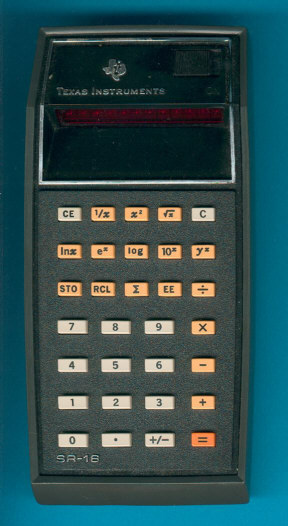
\includegraphics[scale=0.3]{images/sr-16.jpg}
		\end{column}
		\begin{column}{5cm}
			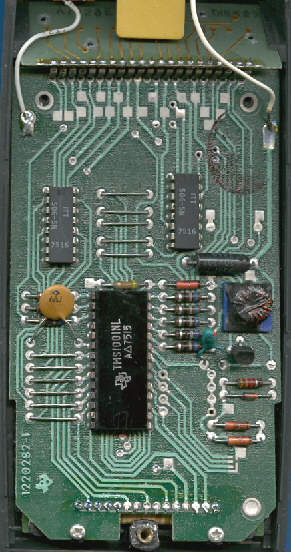
\includegraphics[scale=0.4]{images/SR-16_PCBC.jpg}
		\end{column}
	\end{columns}
\end{frame}		
